\myClearDoublePage
\chapter{Implementation}

The previous section focused on the theoretical approach to designing a tracking module for a receiver, and this chapter will explain the specific practical process and the problems encountered during the process. This project mainly implements the tracking module on a GPS receiver, please note that this is only a separate module and does not realise the full receiver functionality. It also has RF front-end and acquisition modules in the front module, and ranging modules as well as navigation modules in the back module. The project in fact has a hypothetical target device, but based on the current conditions, the main use of VHDL for code writing, as well as behavioural simulation to verify the results, will not be on-board operations.

\section{System Architecture}
\subsection{RF Front-end}

The RF front-end is a device that collects any signals you expect. In this project, we will use \textit{NT1065\_FMC2} as our front-end. This device is designed to receive GPS, GLONASS, Galileo, BeiDou, IRNSS, QZSS and L1, L2, L3, L5, E1, E5a, E5b, E6, B1, B2, B3 bands. It has an FMC(\textit{FPGA Mezzanine Card}) interface, which allows it to have a faster transfer rate to the Xilinx board \cite{RN206}. Figure \ref{fig:nt1065} shows the device's appearance. Here is its key specification table.

\begin{table}[!htbp]
\centering
\caption{Key Specification of \textit{NT1065\_FMC2}}\label{tab:nt1065}
\renewcommand\arraystretch{1.5}
\begin{tabular}{cc}
    \toprule
    Content & Specifications \\
    \midrule
    Chip & NT1065 \\
    Number of channels & 4 \\
    \multirow{2}{*}{Reference frequency sources (MHz)} & TCXO 10 \\
     & TCXO 24.84 \\
    Bit width of ADC (bits) & 2 \\
    \bottomrule
\end{tabular}
\end{table}

\begin{figure}[!htbp]
    \centering
    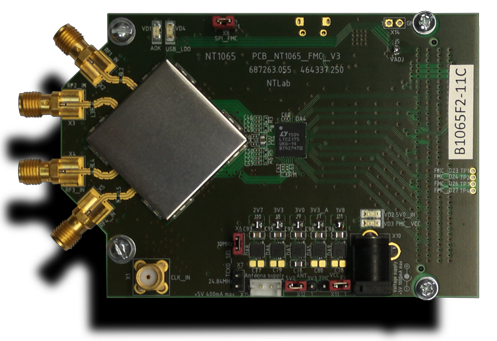
\includegraphics[width=0.8\textwidth]{_IMAGES/fmc-2-nt1065.png}
    \caption{\textit{NT1065\_FMC2}}
    \label{fig:nt1065}
\end{figure}

\subsection{FPGA Board}
The FPGA board is the core module of this project. It will process the acquisition, tracking and navigation stages. The board we choose is \textit{KCU105 Evaluation Board} from \textit{AMD Xilinx}. It's very powerful. Its specification and appearance will be shown below.

\begin{table}[!htbp]
\centering
\caption{Key Specification of KCU105 Evaluation Board}
\label{tab:kcu105}
\renewcommand\arraystretch{1.5}
\begin{tabular}{cc}
    \toprule
    Content & Specifications \\
    \midrule
    Chip & XCKU040-2FFVA1156E FPGA \\
    System Logic Cells (K) & 530 \\
    DSP Slices & 1,920 \\
    Block RAM (Mb) & 21.1 \\
    16.3Gb/s Transceivers & 20 \\
    I/O Pins & 520 \\
    \multirow{3}{*}{Memory} & 2GB DDR4 component memory \\
     & 64MB flash \\
     & 8Kb EEPROM \\
     \bottomrule
\end{tabular}
\end{table}

\begin{figure}[!htbp]
    \centering
    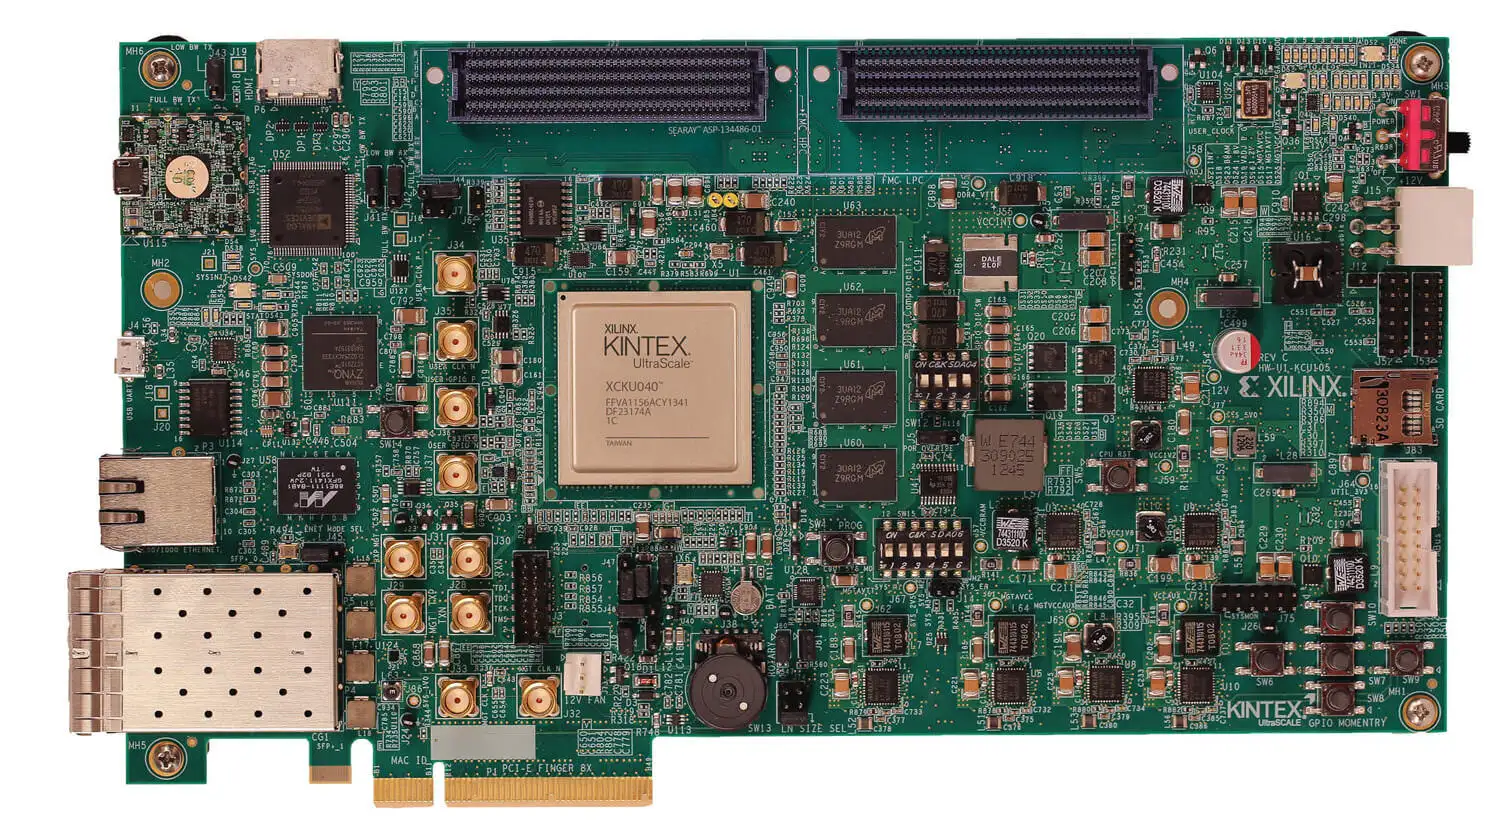
\includegraphics[width=0.8\textwidth]{_IMAGES/KCU105_evaluation_board.png}
    \caption{\textit{KCU105 Evaluation Board}}
    \label{fig:kcu105}
\end{figure}

\section{Develop Environment}
\subsection{Vivado}
As we are planning to use FPGA from \textit{Xilinx}, we are supposed to code in \textit{Vivado}. It is a powerful and versatile integrated development environment (IDE) created by Xilinx for FPGA and SoC development. It offers a comprehensive suite of tools and features for designing, implementing, and programming FPGAs and SoCs, enabling engineers to create custom digital hardware solutions. With its user-friendly interface and advanced design automation capabilities, \textit{Vivado} simplifies the process of hardware design, synthesis, verification, and debugging. It supports a wide range of Xilinx devices, making it a go-to tool for hardware engineers and developers working on cutting-edge applications in industries like telecommunications, aerospace, and embedded systems. The version we use is \textbf{2018.3}. The reason for that is that it is stable but not outdated.

\subsection{ModelSim}
\textit{ModelSim} is used to verify the design. We will run the simulation and check all the waveforms of the key signal. \textit{ModelSim} is a leading digital simulation and verification tool by Mentor Graphics, now a part of Siemens. It's widely used for designing and testing digital systems, enabling engineers to simulate hardware description languages like VHDL and Verilog. \textit{ModelSim} assists in debugging, verification, and validation of complex digital designs in various industries.

\textit{ModelSim} is particularly compatible with Vivado, and when used in conjunction with it, you get twice the result with half the effort, and it can quickly locate code errors.

\subsection{MATLAB}
Matlab is a high-level programming environment and language renowned for its versatility in numerical computing, data analysis, and algorithm development. Used across various fields, from engineering to finance, it offers extensive libraries and tools for modelling, simulation, and solving complex mathematical problems, making it indispensable in research and industry. The reason for using it is to run the \textit{SoftGNSS} to verify my design as well.

\section{Tracking}
Before tracking, we need the acquisition result. The part has been done on the \textit{SoftGNSS}. Here are the results.

\begin{table}[!htbp]
\centering
\caption{Results of the Acquisition}
\label{tab:result_acqu}
\renewcommand\arraystretch{1.5}
\begin{tabular}{cc}
    \toprule
    \multicolumn{2}{c}{Result} \\
    \midrule
    Chopped bits & 46500 \\
    PRN (\textnumero) & 2 \\
    Frequency (MHz) & 14.5778 \\
    Doppler (Hz) & 2200 \\
    Code offset & 162 \\
    \bottomrule
\end{tabular}
\end{table}

These results are fed directly into the tracking stage.

\subsection{NCO}
The NCO block is driven by a 99.375MHz signal. Firstly, we need to obtain the FSW. The bit width of the PA is 32 bits. The required carrier frequency is 